\documentclass[11pt]{article}

\usepackage[margin=1in]{geometry}
\usepackage{booktabs}
\usepackage{graphicx}
\usepackage{hyperref}
\usepackage{natbib}
\usepackage{tabularx}

\title{AnnotateBench: Learning Curves and Cost Frontiers for Annotation Strategy Selection}
\author{Anote AI}
\date{Rough JDSE 2026 Draft}

\begin{document}
\maketitle

\begin{abstract}
Annotation budgets are a practical bottleneck in applied natural language processing, yet teams often choose labeling strategies without direct evidence about expected accuracy gains, diminishing returns, or cost tradeoffs. We introduce AnnotateBench, a benchmark framework for comparing annotation strategies through downstream learning curves, cost-performance frontiers, and budget recommendations. The current JDSE 2026 rough draft reports an initial pilot using public gold-labeled datasets rather than newly collected human annotations. In the pilot, annotation is simulated by revealing labels from the training split according to each selection strategy. We compare random sampling, uncertainty-based active learning, diversity-based active learning, and a hybrid strategy across Financial PhraseBank, TREC, and Banking77 using a common TF-IDF logistic-regression classifier. The intended contribution is not a final leaderboard, but a reproducible empirical scaffold for measuring how many labeled examples are needed to reach strong downstream performance under different annotation strategies.
\end{abstract}

\section{Introduction}

Labeled data remains one of the most expensive inputs to real-world NLP systems. Even when model architectures and training code are standardized, teams still need to decide which examples to annotate, how large an initial labeling batch should be, and when further annotation is no longer worth the marginal cost. These decisions are often made using rules of thumb or isolated active-learning experiments rather than a benchmark that directly compares annotation strategies under a shared budget and evaluation protocol.

AnnotateBench addresses the following question: how do different annotation strategies perform across NLP tasks and label budgets, and how many labeled examples are needed to reach strong downstream performance? The benchmark is designed around learning curves rather than single-budget scores. For each strategy, it evaluates downstream performance as a function of labeled examples, estimates annotation cost, and identifies Pareto-efficient budget-strategy choices.

The paper is motivated by prior Anote work showing that labeling a small number of high-value examples can improve classification performance across datasets such as Financial PhraseBank, Banking, Craigslist, TREC, and Amazon Reviews \citep{vidra2024humanfeedback}. AnnotateBench extends that idea into a systematic benchmark across annotation strategies, datasets, label budgets, and cost-performance tradeoffs. The first implementation intentionally uses public datasets with existing gold labels and simulates annotation budgets by subsampling labeled training examples selected by each strategy. This design avoids new human-subject data collection while preserving the core experimental question: which examples would an annotation process choose under a fixed budget, and what downstream model quality would those labels support?

This rough draft targets JDSE 2026 and should be read as a pilot manuscript. Its immediate scope is three text-classification datasets, five label budgets, four selection strategies, a TF-IDF logistic-regression downstream model, and scenario-based annotation cost assumptions. The full benchmark will extend this grid to stronger models, more repetitions, calibrated annotation costs, and LLM-assisted annotation baselines.

\section{Related Work}

\subsection{Data-Centric AI Benchmarks}

Recent benchmark work argues that progress in applied AI depends not only on model architecture, but also on how data is acquired, filtered, labeled, and evaluated. DataPerf formalizes data-centric AI evaluation through benchmark tasks for data selection, debugging, acquisition, and related dataset-improvement workflows \citep{mazumder2022dataperf}. Data acquisition benchmarks further emphasize transparent pricing, standardized data formats, and realistic interactions between data providers and consumers \citep{chen2023dataacquisition}. DataComp makes a related point at multimodal scale: dataset filtering and curation can be benchmarked under standardized training and evaluation pipelines \citep{gadre2023datacomp}. AnnotateBench follows this data-centric benchmark tradition, but focuses specifically on label-budget allocation for NLP annotation strategies.

Data valuation work is also closely related because it asks which individual examples are useful for model training. Dataset Cartography uses training dynamics to identify easy, ambiguous, and hard-to-learn examples in NLP datasets \citep{swayamdipta2020dataset}. OpenDataVal provides a unified benchmark for data valuation algorithms across image, natural-language, and tabular tasks \citep{jiang2023opendataval}. Transferred Shapley approaches adapt data valuation to fine-tuning large language models \citep{schoch2023dataselection}. AnnotateBench differs by evaluating examples at the moment they would be selected for annotation, before their labels are assumed to be available.

\subsection{LLM-Assisted Annotation}

Large language models have made automated and semi-automated annotation a live empirical question rather than a speculative future direction. Wang et al. show that GPT-3-generated labels can substantially reduce labeling costs for downstream NLP tasks, especially when combined with limited human labels \citep{wang2021gpt3labeling}. A recent survey organizes the area around LLM-generated annotations, assessment of those annotations, and downstream use of LLM-labeled data \citep{tan2024llmannotation}. Empirical studies report that LLM labels can be competitive with human labels for some text-annotation tasks \citep{gilardi2023chatgpt}, that LLM-generated training labels can support supervised text classifiers across computational social science tasks \citep{pangakis2024distillation}, and that teacher-student pipelines can use GPT-labeled data to train smaller multilingual news-topic classifiers \citep{kuzman2024teacherstudent}. These results motivate including LLM annotation in the full AnnotateBench grid, but they also show why LLM baselines must be versioned, costed, and evaluated under the same budget protocol as human annotation strategies.

\subsection{Few-Shot Classification with Human Feedback}

AnnotateBench is closest in spirit to recent work on improving classification with a small number of labeled examples. Vidra et al. evaluate a continuous human-feedback loop across Financial PhraseBank, Banking, Craigslist, TREC, and Amazon Reviews, using models such as GPT-3.5, BERT, and SetFit \citep{vidra2024humanfeedback}. SetFit is especially relevant because it demonstrates strong few-shot text classification without prompt engineering or very large models \citep{tunstall2022setfit}. AnnotateBench builds on this line of work by turning the feedback loop into a benchmark question: at each budget, which strategy should choose the examples, what does that strategy cost, and where does it sit on the learning curve?

\subsection{Human-in-the-Loop and Active Annotation}

The most relevant recent work is no longer only classic uncertainty sampling; it is the combination of active selection, LLM-generated labels, and selective human review. Rouzegar and Makrehchi integrate LLM outputs with human annotation inside an active-learning framework and explicitly optimize cost-performance tradeoffs for text classification \citep{rouzegar2024llmdriven}. This line of work is close to AnnotateBench's motivation, but it is primarily method-specific. AnnotateBench is positioned as a benchmark layer: it compares multiple annotation strategies, budget levels, and cost frontiers under one reproducible protocol.

\subsection{Expert, Span, and Domain-Specific Annotation}

Newer LLM annotation work also cautions against treating LLM labeling as uniformly solved. Span-annotation studies find that LLMs can be cost-efficient and sometimes comparable to skilled annotators, but agreement varies by task and model type \citep{kasner2025spanannotators}. Expert-domain evaluations report mixed results in finance, biomedicine, and law, including limited gains from reasoning-style inference-time techniques in some settings \citep{tseng2025expertannotators}. AnnotateBench therefore treats LLM annotation as a strategy family whose cost, reliability, and domain sensitivity must be benchmarked rather than assumed.

\subsection{Pilot Datasets}

The pilot uses Financial PhraseBank, a financial sentiment dataset with positive, neutral, and negative labels \citep{malo2014good}. It is a strong first dataset because it is small, domain-specific, and aligned with the motivating classification use case. Candidate next datasets include TREC question classification \citep{li2002learning} and Banking77 intent classification \citep{casanueva2020efficient}. These additions would test whether observed budget recommendations transfer beyond financial sentiment.

\begin{table}[t]
\centering
\caption{Literature review and novelty positioning. Recent work motivates evaluating annotation as a data-centric, cost-sensitive benchmark problem rather than only as a classic active-learning algorithm comparison.}
\label{tab:literature-novelty}
\small
\begin{tabularx}{\textwidth}{p{0.20\textwidth}p{0.24\textwidth}p{0.25\textwidth}X}
\toprule
Work or area & Main focus & Typical evidence & AnnotateBench distinction \\
\midrule
DataPerf and data acquisition \citep{mazumder2022dataperf,chen2023dataacquisition} & Benchmark data-centric AI workflows. & Standardized data tasks, acquisition settings, and reproducible submissions. & Narrows the benchmark target to NLP annotation strategy selection and label-budget tradeoffs. \\
DataComp \citep{gadre2023datacomp} & Benchmark dataset filtering and curation at scale. & Standardized training code and downstream evaluations. & Adopts the same benchmark philosophy for labeled-example selection rather than web-scale multimodal filtering. \\
Data valuation \citep{swayamdipta2020dataset,jiang2023opendataval,schoch2023dataselection} & Estimate which examples are valuable or harmful for model training. & Data-value scores and downstream retraining results. & Measures value through annotation-time selection under explicit label budgets. \\
Prior Anote feedback study \citep{vidra2024humanfeedback} & Improve classification with a few human-labeled examples. & Iterative feedback results across several text-classification datasets. & Extends the idea into strategy comparisons, learning curves, and cost frontiers. \\
LLM annotation surveys \citep{tan2024llmannotation} & Taxonomize LLM-based annotation, assessment, and use. & Survey of methods and failure modes. & Converts the taxonomy into measurable strategy-budget comparisons. \\
LLM labels for classifiers \citep{wang2021gpt3labeling,pangakis2024distillation,kuzman2024teacherstudent} & Replace or augment human labels with model-generated labels. & Downstream classifier performance using LLM-generated training data. & Evaluates LLM labels as one costed strategy rather than the only intervention. \\
Few-shot classifiers \citep{tunstall2022setfit} & Learn accurate classifiers from few labeled examples. & Few-shot accuracy under lightweight fine-tuning. & Uses such models as possible downstream learners while benchmarking annotation choices. \\
LLM + human active annotation \citep{rouzegar2024llmdriven} & Combine selection policies, LLM labels, and human review. & Cost-performance results on selected text tasks. & Generalizes the question into a reusable benchmark grid across strategies and budgets. \\
Expert and span-level LLM annotation \citep{kasner2025spanannotators,tseng2025expertannotators} & Test LLMs on span and expert-domain annotation tasks. & Agreement, cost, and domain-specific annotation quality. & Treats reliability and domain sensitivity as benchmark dimensions for later versions. \\
Pilot classification datasets \citep{malo2014good,li2002learning,casanueva2020efficient} & Provide public gold labels for task evaluation. & Task-level model scores. & Reuses gold labels to simulate annotation budgets without new human-subject data collection. \\
\bottomrule
\end{tabularx}
\end{table}

\section{Methodology}

\subsection{Problem Setup}

Let $D_{\mathrm{train}}=\{(x_i,y_i)\}_{i=1}^{n}$ denote a public training set with gold labels and let $D_{\mathrm{test}}$ denote a held-out test set. An annotation strategy $s$ receives access to the unlabeled training inputs and a budget $b$. The strategy selects a subset $S_{s,b}$ of at most $b$ training examples. The experiment reveals the gold labels for those selected examples, trains a downstream classifier on $S_{s,b}$, and evaluates the classifier on $D_{\mathrm{test}}$.

This setup simulates the outcome of annotation without collecting new human labels. It does not measure human annotation time, disagreement, fatigue, or interface effects. It does, however, isolate the budgeted selection question that arises before annotation begins.

\subsection{Annotation Strategies}

The current pilot compares four strategies:

\begin{itemize}
  \item \textbf{Random sampling}: select examples uniformly at random from the training pool.
  \item \textbf{Uncertainty active learning}: seed the labeled set with class coverage, train an interim model, and select high-entropy examples.
  \item \textbf{Diversity active learning}: select examples to improve coverage in TF-IDF feature space.
  \item \textbf{Hybrid active learning}: combine a diversity-oriented seed with uncertainty-based selection.
\end{itemize}

The planned full benchmark may add LLM-assisted annotation, simulated noisy annotation, and additional active-learning algorithms. These are excluded from the current empirical claims until their cost and quality assumptions are explicit.

\subsection{Learning Curves}

For each strategy and budget, AnnotateBench records macro F1 and accuracy. The main analysis plots macro F1 against the number of revealed labels. Learning curves make two quantities visible that single-budget reporting hides: the early-budget slope and the point of diminishing returns. In the full paper, these curves should support budget recommendations such as the smallest budget that reaches a target macro F1 or the lowest-cost Pareto-efficient configuration.

\subsection{Cost and Pareto Frontiers}

The pilot treats annotation cost as a sensitivity parameter rather than a fixed fact. We report low, base, and high human-label cost scenarios with per-label costs of \$0.03, \$0.10, and \$0.30, respectively. The base scenario also includes a small illustrative selection overhead for active-learning strategies: \$0.002 per example for uncertainty sampling, \$0.003 for diversity sampling, and \$0.004 for the hybrid strategy. Random sampling has no selection overhead. For a strategy $s$, budget $b$, human-label cost $h$, and selection overhead $o_s$, estimated cost is
\[
  C(s,b)=(h + o_s) \times |S_{s,b}|.
\]
A budget-strategy point is Pareto-efficient if no other point has both lower or equal cost and higher or equal macro F1, with at least one strict improvement. Pareto frontiers are intended to help practitioners compare strategy choices under realistic budget constraints. The current figures use the base scenario; the result CSVs retain all three cost scenarios for sensitivity analysis.

\section{Experiment Setup}

\subsection{Dataset}

The pilot includes Financial PhraseBank \citep{malo2014good}, TREC coarse question classification \citep{li2002learning}, and Banking77 intent classification \citep{casanueva2020efficient}. Financial PhraseBank is a three-way financial sentiment task; the loader creates a deterministic stratified 80/20 train/test split using random seed 42. TREC uses the public coarse-label train/test split. Banking77 uses the public intent-classification train/test split with 77 classes.

\subsection{Model and Metrics}

Each condition trains the same downstream text classifier: TF-IDF features with unigram and bigram features followed by logistic regression. Macro F1 is the primary metric because class imbalance can obscure poor minority-class performance. Accuracy is retained as a secondary metric for interpretability.

\subsection{Budget Grid and Repetition}

The pilot budget grid is 50, 100, 250, 500, and 1000 labeled examples, capped at the available training set size. The current draft reports three strategy-selection seeds, 0, 1, and 2. The final paper should expand this repetition, add confidence intervals, and report sensitivity to train/test split choices where feasible.

\subsection{Reproducible Outputs}

The expected pilot artifacts are:

\begin{itemize}
  \item \texttt{results/pilot\_results.csv}: Financial PhraseBank results.
  \item \texttt{results/pilot\_results\_trec.csv}: TREC results.
  \item \texttt{results/pilot\_results\_banking77.csv}: Banking77 results.
  \item \texttt{results/budget\_recommendations.csv}: cheapest strategy-budget pairs for target macro F1 thresholds under the base cost scenario.
  \item \texttt{figures/learning\_curve\_*.png} and \texttt{figures/pareto\_*.png}: learning curves and base-scenario cost frontiers for each pilot dataset.
\end{itemize}

\section{Preliminary Results}

The current pilot uses three strategy-selection seeds, 0, 1, and 2. Table~\ref{tab:pilot-results} summarizes the best mean macro F1 for each dataset-strategy pair under the base cost scenario. The ranking varies by dataset: uncertainty sampling is best on Financial PhraseBank, while random sampling is best on TREC and Banking77 under this simple TF-IDF logistic-regression setup.

\begin{table}[h]
\centering
\caption{Pilot results under the base cost scenario. Scores are mean macro F1 $\pm$ sample standard deviation over three strategy-selection seeds.}
\label{tab:pilot-results}
\begin{tabular}{llrrr}
\toprule
Dataset & Strategy & Best macro F1 & Budget & Base cost \\
\midrule
Financial PhraseBank & Uncertainty AL & 0.809 $\pm$ 0.007 & 1000 & \$102.00 \\
Financial PhraseBank & Hybrid AL & 0.800 $\pm$ 0.007 & 1000 & \$104.00 \\
Financial PhraseBank & Random & 0.749 $\pm$ 0.021 & 1000 & \$100.00 \\
Financial PhraseBank & Diversity AL & 0.561 $\pm$ 0.053 & 1000 & \$103.00 \\
TREC & Random & 0.668 $\pm$ 0.044 & 1000 & \$100.00 \\
TREC & Uncertainty AL & 0.655 $\pm$ 0.100 & 1000 & \$102.00 \\
TREC & Hybrid AL & 0.504 $\pm$ 0.022 & 1000 & \$104.00 \\
TREC & Diversity AL & 0.485 $\pm$ 0.009 & 1000 & \$103.00 \\
Banking77 & Random & 0.446 $\pm$ 0.021 & 1000 & \$100.00 \\
Banking77 & Diversity AL & 0.330 $\pm$ 0.014 & 1000 & \$103.00 \\
Banking77 & Hybrid AL & 0.167 $\pm$ 0.043 & 1000 & \$104.00 \\
Banking77 & Uncertainty AL & 0.158 $\pm$ 0.029 & 1000 & \$102.00 \\
\bottomrule
\end{tabular}
\end{table}

Table~\ref{tab:budget-recommendations} shows budget recommendations for representative target macro F1 thresholds under the base cost scenario. Several thresholds are not reached, especially on Banking77, which is expected because the 77-class intent task is difficult at the current budget range with a simple linear model.

\begin{table}[h]
\centering
\caption{Cheapest strategy-budget pairs for selected target macro F1 thresholds under the base cost scenario. Blank entries indicate that no strategy reached the target in the pilot grid.}
\label{tab:budget-recommendations}
\begin{tabular}{llrrr}
\toprule
Dataset & Target F1 & Strategy & Budget & Base cost \\
\midrule
Financial PhraseBank & 0.50 & Hybrid AL & 50 & \$5.20 \\
Financial PhraseBank & 0.70 & Hybrid AL & 500 & \$52.00 \\
Financial PhraseBank & 0.80 & Uncertainty AL & 1000 & \$102.00 \\
TREC & 0.50 & Random & 500 & \$50.00 \\
TREC & 0.60 & Random & 500 & \$50.00 \\
TREC & 0.70 & -- & -- & -- \\
Banking77 & 0.30 & Random & 1000 & \$100.00 \\
Banking77 & 0.50 & -- & -- & -- \\
\bottomrule
\end{tabular}
\end{table}

These pilot results support the benchmark framing rather than a universal strategy claim. The best strategy changes across datasets, and the active-learning variants are not automatically better than random sampling under small budgets and sparse TF-IDF features. This matters for annotation planning: strategy choice should be evaluated jointly with task, budget, model family, and cost assumptions.

\begin{figure}[h]
\centering
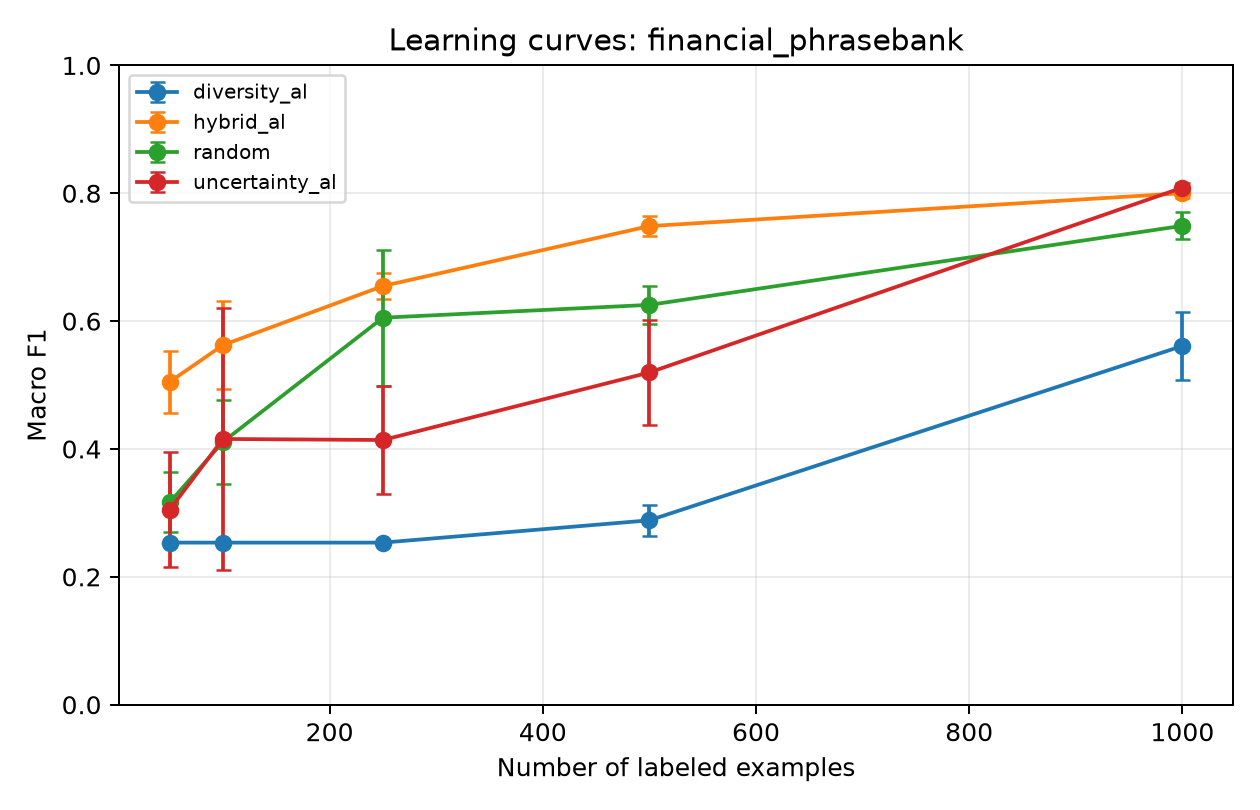
\includegraphics[width=0.86\textwidth]{../figures/learning_curve_financial_phrasebank.png}
\caption{Learning curves for the Financial PhraseBank pilot.}
\label{fig:learning-curve-financial}
\end{figure}

\begin{figure}[h]
\centering
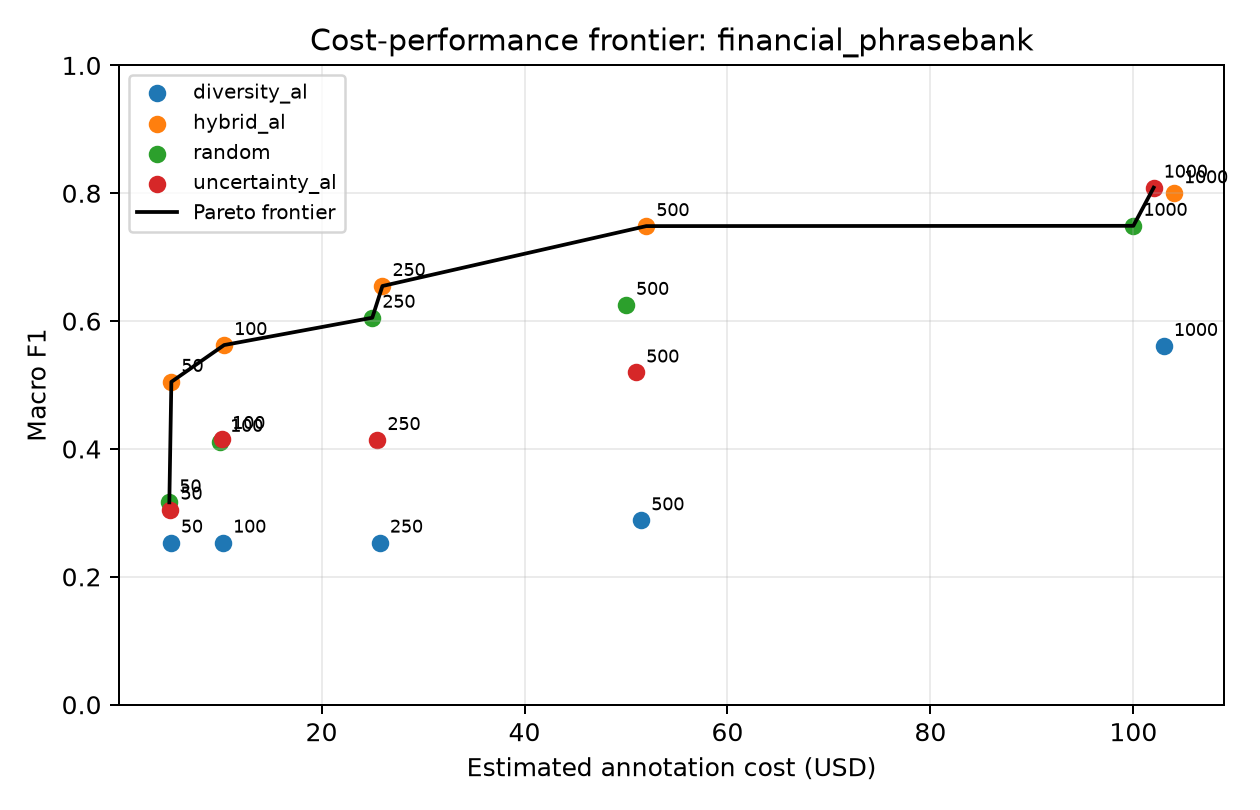
\includegraphics[width=0.86\textwidth]{../figures/pareto_financial_phrasebank.png}
\caption{Cost-performance Pareto frontier for the Financial PhraseBank pilot.}
\label{fig:pareto-financial}
\end{figure}

\begin{figure}[h]
\centering
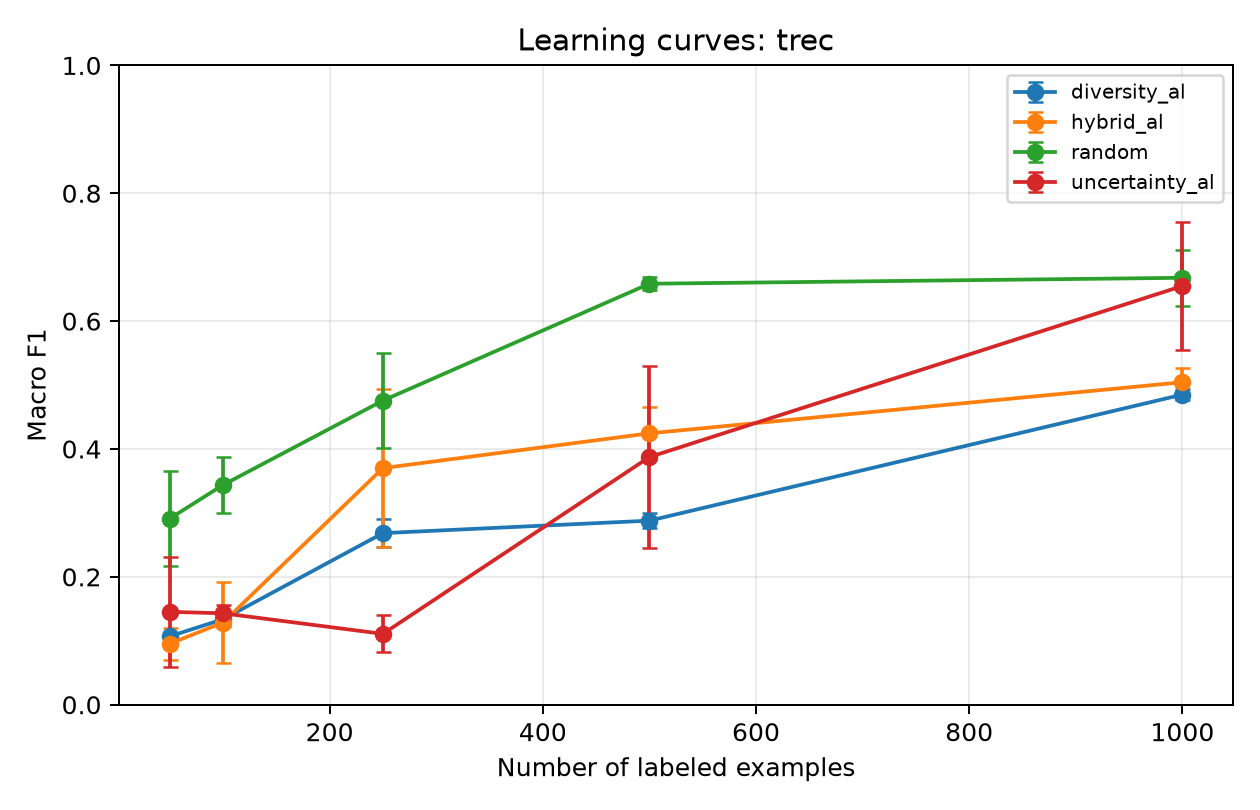
\includegraphics[width=0.86\textwidth]{../figures/learning_curve_trec.png}
\caption{Learning curves for the TREC pilot.}
\label{fig:learning-curve-trec}
\end{figure}

\begin{figure}[h]
\centering
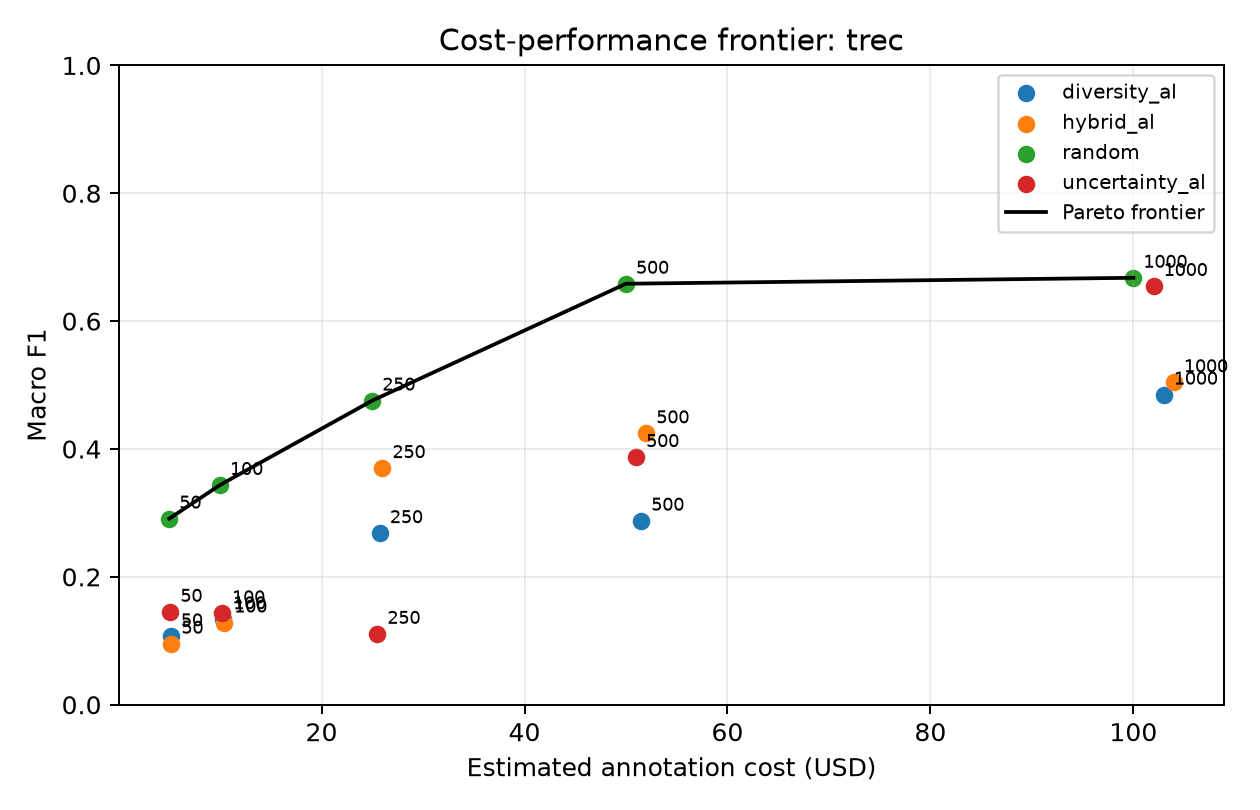
\includegraphics[width=0.86\textwidth]{../figures/pareto_trec.png}
\caption{Cost-performance Pareto frontier for the TREC pilot under the base cost scenario.}
\label{fig:pareto-trec}
\end{figure}

\begin{figure}[h]
\centering
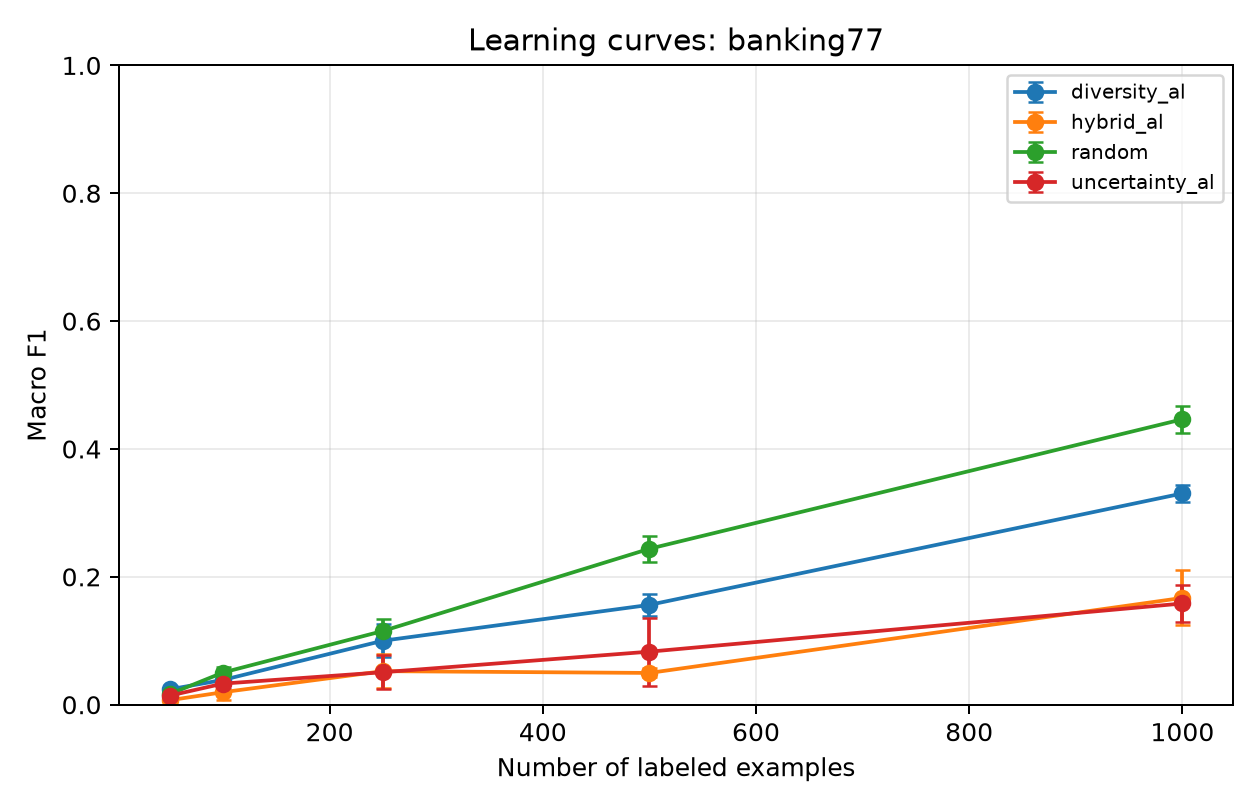
\includegraphics[width=0.86\textwidth]{../figures/learning_curve_banking77.png}
\caption{Learning curves for the Banking77 pilot.}
\label{fig:learning-curve-banking77}
\end{figure}

\begin{figure}[h]
\centering
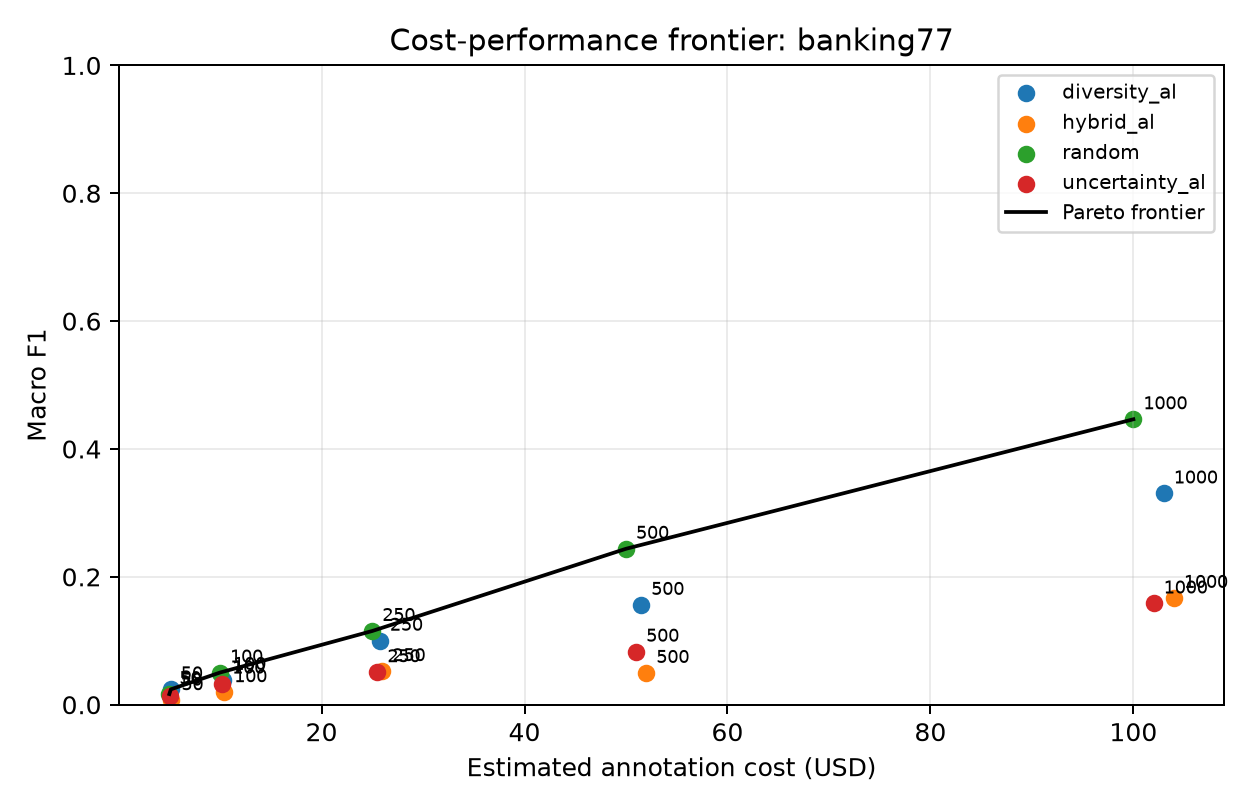
\includegraphics[width=0.86\textwidth]{../figures/pareto_banking77.png}
\caption{Cost-performance Pareto frontier for the Banking77 pilot under the base cost scenario.}
\label{fig:pareto-banking77}
\end{figure}

\section{Limitations}

The current draft has several important limitations. First, it reports only three strategy-selection seeds rather than final empirical results with confidence intervals. Second, the downstream model is intentionally simple; stronger neural or instruction-tuned models may change the shape of the learning curves. Third, the cost model is scenario-based but still illustrative: it does not yet use measured annotation platform pricing, LLM API prices, selection runtime, annotation latency, quality control, or annotator disagreement. Fourth, gold-label simulation does not capture the full process of human annotation, including ambiguous examples and inconsistent labeler behavior. Fifth, LLM-assisted annotation is discussed as related and planned work but is not yet included as a measured strategy.

\section{Next Steps}

The next manuscript milestone is to strengthen the current three-dataset pilot. The most important additions are:

\begin{itemize}
  \item run more seeds and report confidence intervals;
  \item calibrate human annotation and LLM annotation cost assumptions against external pricing sources;
  \item decide whether the LLM annotator baseline is a noisy-label simulator, a zero-shot prompted model, or deferred entirely;
  \item compare against at least one stronger downstream learner;
  \item run ablations on active-learning warm-start size and representation choice.
\end{itemize}

\section{Conclusion}

AnnotateBench frames annotation strategy selection as an empirical budget-allocation problem. Instead of asking only which model achieves the highest score, it asks how performance improves as labels are revealed and which strategy-budget combinations are cost-efficient. The current JDSE 2026 draft establishes the paper structure, pilot methodology, novelty positioning, and first three-dataset evidence needed to turn the repository's experiment outputs into a complete benchmark paper.

\bibliographystyle{plainnat}
\bibliography{references}

\end{document}
